%% =====================================================================
%% Control Valve Sizing Assignment - revised version
%%
%% OPEN POINTS (everything marked red [..] in the PDF must be filled in):
%%  1. Re-run Nelprof (RE + M1) with the NEW input data of Table 2
%%     (inlet 1.55 barG, outlet 0.20 barG, dp 1.35 bar, DPm = 0.97 in the
%%     chart/process-model settings!) and fill in the macros below.
%%  2. Replace the Nelprof screenshots in "Pictures Nelprof/" (setup,
%%     installed characteristic, gain, pressure level, noise) and add a
%%     screenshot showing where DPm = 0.97 is entered.
%%     (Inherent-characteristic figures stay valid - they do not depend on DPm.)
%%  3. Check retrieval date / URL of "Pressure Drop Online" and Nelprof.
%%  4. Check the AI declaration: it must describe what YOU really did.
%% =====================================================================
\documentclass[11pt,a4paper]{article}

% ----- Encoding & Language -----
\usepackage[utf8]{inputenc}
\usepackage[T1]{fontenc}
\usepackage{lmodern}
\usepackage[english]{babel}

% ----- Layout & Formatting -----
\usepackage[margin=2.5cm]{geometry}
\usepackage{graphicx}
\usepackage{xcolor}
\usepackage{amsmath}
\usepackage{amssymb}
\usepackage{booktabs}
\usepackage{tabularx}
\usepackage{caption}
\usepackage{hyperref}
\usepackage{fancyhdr}
\usepackage{float}
\usepackage{enumitem}
\usepackage{tikz}
\usetikzlibrary{arrows.meta,calc,decorations.pathreplacing}
\captionsetup{font=small,labelfont=bf}
\setlength{\parindent}{0pt}
\setlength{\parskip}{0.6em}
\setlength{\headheight}{14pt}
\emergencystretch=3em
\Urlmuskip=0mu plus 1mu\relax

% ----- Header & Footer -----
\pagestyle{fancy}
\fancyhf{}
\fancyhead[L]{Control Valve Sizing Assignment}
\fancyhead[R]{Mathias Lampert}
\fancyfoot[C]{\thepage}
\renewcommand{\headrulewidth}{0.4pt}

% ----- Placeholder for Nelprof results that must be re-run -----
\newcommand{\nel}[1]{\textcolor{red}{\textbf{[#1]}}}
% RE-series results
\newcommand{\REcv}{\nel{RE Cv}}
\newcommand{\REtravel}{\nel{RE travel \%}}
\newcommand{\REangle}{\nel{RE angle}}
\newcommand{\REnoise}{\nel{RE dBA}}
\newcommand{\REchoked}{\nel{RE choked dp}}
\newcommand{\REflowhalf}{\nel{flow at 0.5 travel}}
\newcommand{\REflowhigh}{\nel{flow at 0.8 travel}}
\newcommand{\REgmin}{\nel{RE Gmin}}
\newcommand{\REgmax}{\nel{RE Gmax}}
\newcommand{\REratio}{\nel{RE Gmax/Gmin}}
\newcommand{\REnoisepeak}{\nel{RE peak dBA}}
\newcommand{\REnoisepeaktravel}{\nel{at travel \%}}
\newcommand{\REpinfull}{\nel{rel. inlet p, valve open}}
% M1-series results
\newcommand{\Mcv}{\nel{M1 Cv}}
\newcommand{\Mtravel}{\nel{M1 travel \%}}
\newcommand{\Mangle}{\nel{M1 angle}}
\newcommand{\Mnoise}{\nel{M1 dBA}}
\newcommand{\Mnoisepeak}{\nel{M1 peak dBA}}
\newcommand{\Mnoisepeaktravel}{\nel{at travel \%}}
\newcommand{\Mchoked}{\nel{M1 choked dp}}
\newcommand{\Mtraveleighty}{\nel{travel at 80 \% flow}}
\newcommand{\Mtravelninety}{\nel{travel at 90 \% flow}}
\newcommand{\Mgmin}{\nel{M1 Gmin}}
\newcommand{\Mgmax}{\nel{M1 Gmax}}
\newcommand{\Mgop}{\nel{M1 G at op. point}}
\newcommand{\Mratio}{\nel{M1 Gmax/Gmin}}
\newcommand{\Mpinfull}{\nel{rel. inlet p, valve open}}

\begin{document}

% ---------------------------------------------------------
% Title page
\begin{titlepage}
\centering
\vspace*{3cm}
{\Huge\bfseries Control Valve Sizing Assignment\par}
\vspace{0.8cm}
{\Large Field Devices and Instrumentation\par}
\vspace{0.5cm}
{\large Process application: LAA01AA202 -- circulation from the pressure tank back to the pressure tank\par}
\vspace{3cm}
{\large Mathias Lampert\par}
\vspace{0.5cm}
{\large October 2026\par}
\vfill
{\small JAMK University of Applied Sciences}
\end{titlepage}

\tableofcontents
\clearpage
\listoffigures
\listoftables
\clearpage

% ---------------------------------------------------------
\section{Introduction}
The objective of this assignment is to perform a complete control valve sizing exercise for a closed-loop water circulation process. By evaluating the pump curve and calculating the pressure loss between the pump and the valve, the pressure drop across the valve is determined and a suitable valve is sized with Valmet Nelprof. The report compares the currently installed valve type (represented by the Valmet M1-series) with an RE-series segmented ball valve, based on flow control theory (JAMK University of Applied Sciences, 2024; Valmet, 2022), and justifies the final selection.

% ---------------------------------------------------------
\section{Process Application Description}
The assigned process (valve position LAA01AA202) is a continuous closed-loop water circulation: water at $25^\circ\text{C}$ is pumped from the $0.2\,\text{m}^3$ pressure tank (LAA01BB001) by pump LAA01AP201 and returned to the same tank through the control valve (Figure~\ref{fig:pid}). The section under consideration runs from the pump discharge to the tank inlet; its layout is shown schematically in Figure~\ref{fig:sketch}.

\begin{figure}[H]
    \centering
    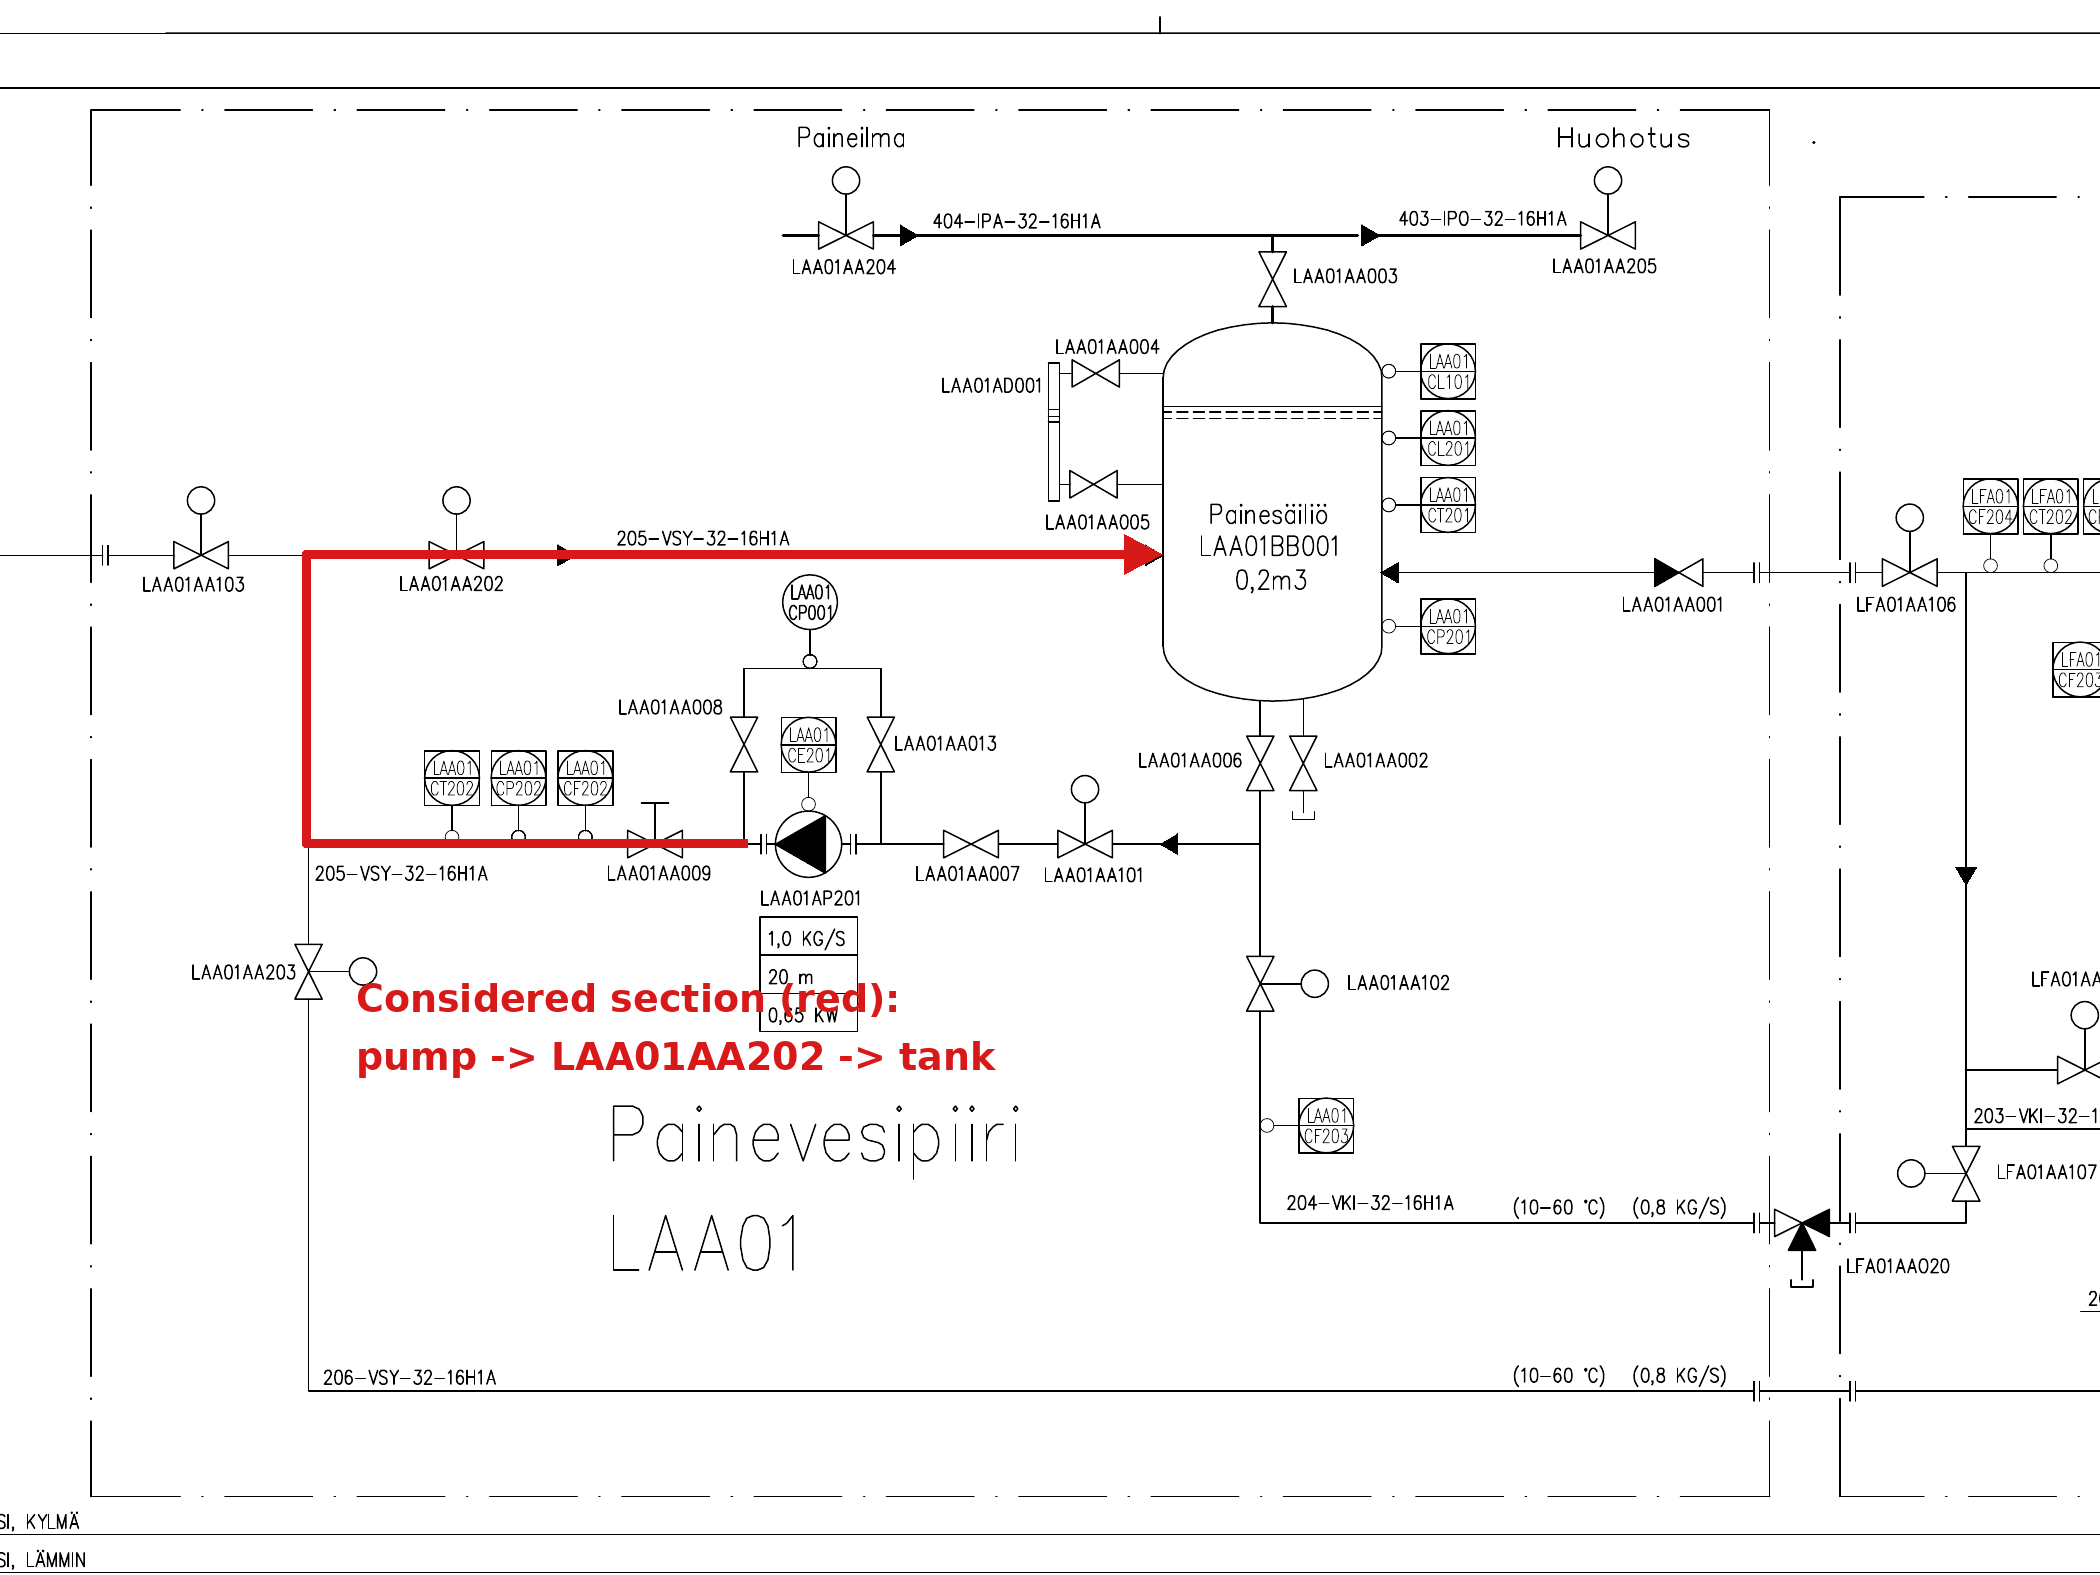
\includegraphics[width=\textwidth]{Pictures/PID_Excerpt_LAA01AA202.png}
    \caption{P\&I diagram excerpt of the pressure water circuit LAA01 with the considered section marked in red. \textit{Note.} Adapted from JAMK University of Applied Sciences (n.d.).}
    \label{fig:pid}
\end{figure}

\begin{figure}[H]
    \centering
    \resizebox{\textwidth}{!}{%
    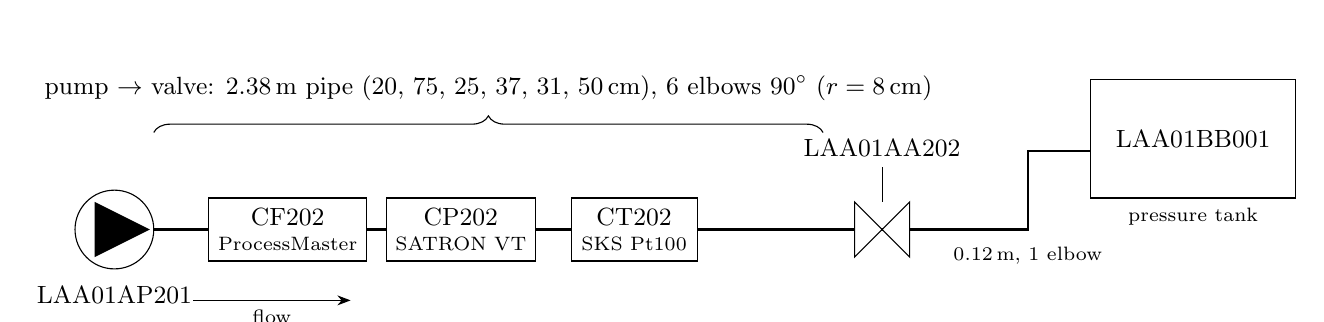
\begin{tikzpicture}[>=Stealth, every node/.style={font=\small}]
        % pump
        \draw (0,0) circle (0.5);
        \fill (-0.25,0.35) -- (-0.25,-0.35) -- (0.45,0) -- cycle;
        \node[below=0.6cm] at (0,0) {LAA01AP201};
        % pipe and instruments
        \draw[thick] (0.5,0) -- (11,0);
        \node[draw,fill=white,minimum width=1.6cm,minimum height=0.8cm,align=center] (cf) at (2.2,0) {CF202\\[-2pt]\scriptsize ProcessMaster};
        \node[draw,fill=white,minimum width=1.6cm,minimum height=0.8cm,align=center] (cp) at (4.4,0) {CP202\\[-2pt]\scriptsize SATRON VT};
        \node[draw,fill=white,minimum width=1.6cm,minimum height=0.8cm,align=center] (ct) at (6.6,0) {CT202\\[-2pt]\scriptsize SKS Pt100};
        % brace over the pump->valve section
        \draw[decorate,decoration={brace,amplitude=6pt,raise=18pt}] (0.5,0.6) -- (9.0,0.6)
            node[midway,above=26pt,align=center] {pump $\rightarrow$ valve: 2.38\,m pipe (20, 75, 25, 37, 31, 50\,cm), 6 elbows $90^\circ$ ($r=8$\,cm)};
        % valve
        \draw[fill=white] (9.4,0.35) -- (9.4,-0.35) -- (10.1,0.35) -- (10.1,-0.35) -- cycle;
        \draw (9.75,0.35) -- (9.75,0.8) node[above] {LAA01AA202};
        % downstream
        \draw[thick] (11,0) -- (11.6,0) -- (11.6,1.0) -- (12.4,1.0);
        \node[below] at (11.6,-0.1) {\scriptsize 0.12\,m, 1 elbow};
        % tank
        \draw (12.4,0.4) rectangle (15.0,1.9);
        \node at (13.7,1.15) {LAA01BB001};
        \node[below] at (13.7,0.4) {\scriptsize pressure tank};
        % flow arrows
        \draw[->] (1.0,-0.9) -- (3.0,-0.9) node[midway,below] {\scriptsize flow};
    \end{tikzpicture}}
    \caption{Schematic (not to scale) of the section pump $\rightarrow$ valve $\rightarrow$ tank. Instrument order as in the P\&I diagram.}
    \label{fig:sketch}
\end{figure}

\textbf{Current installation (baseline):}
\begin{itemize}
    \item \textbf{Pump:} Kolmeks L-32A/2 centrifugal pump, $105\,\text{mm}$ impeller, 3-phase motor, $50\,\text{Hz}$ (3000\,r/min), DN\,32.
    \item \textbf{Current valve:} Jamesbury 25-716D-31-3600XTZ2 ball valve (DN\,25, PN16), design pressure up to $500\,\text{kPa}$, design temperature up to $120^\circ\text{C}$, design flow range $0$--$0.8\,\text{kg/s}$ according to the device description of LAA01AA202.
    \item \textbf{Current actuator:} AUMA electric part-turn actuator SGR\,04.3.
    \item \textbf{Flow requirement:} design operating flow $q = 0.85\,\text{l/s}$ ($3.06\,\text{m}^3/\text{h}$, $3060\,\text{kg/h}$). This is about 6\,\% above the upper end of the documented valve design range of $0.8\,\text{kg/s}$.
\end{itemize}

% ---------------------------------------------------------
\section{Calculations and Sizing Methodology}

\subsection{Input Data and Assumptions}
Table~\ref{tab:input} lists the input data; the assumptions made in the calculation are listed below it.

\begin{table}[H]
\centering
\caption{Input data}
\label{tab:input}
\small
\begin{tabularx}{\textwidth}{@{}lXl@{}}
\toprule
Quantity & Value & Source \\
\midrule
Medium, temperature & Water, $25^\circ\text{C}$ & Assignment data \\
Design flow $q$ & $0.85\,\text{l/s} = 3.06\,\text{m}^3/\text{h}$ & Assignment data \\
Density $\rho$ / kinematic viscosity $\nu$ & $1000\,\text{kg/m}^3$ / $0.893\,\text{mm}^2/\text{s}$ & Assumption / water at $25^\circ\text{C}$ \\
Vapour pressure $p_v$ & $0.0317\,\text{bar(a)}$ & Nelprof (water, $25^\circ\text{C}$) \\
Pipe (pump to tank) & DN\,32, $d = 32\,\text{mm}$, steel, $\varepsilon = 0.046\,\text{mm}$ & P\&I diagram (JAMK, n.d.) \\
Pump & Kolmeks L-32A/2, $\varnothing 105\,\text{mm}$, $50\,\text{Hz}$ & Kolmeks (2012) \\
Pump head at $q$ / shut-off head & $H = 14\,\text{m}$ / $H_0 = 14.2\,\text{m}$ & Kolmeks (2012), Figure~\ref{fig:pump} \\
Tank pressure $p_{tank}$ & $0.2\,\text{barG}$ (assumed) & Assumption \\
Valve candidates & RE-series DN\,25 PN40, M1-series DN\,25 PN40 & Assignment data \\
\bottomrule
\end{tabularx}
\end{table}

\textbf{Assumptions:}
\begin{enumerate}[label=A\arabic*,leftmargin=*,nosep]
    \item Only the section pump $\rightarrow$ valve $\rightarrow$ tank is considered, as required by the assignment. Suction-side losses and static head differences are neglected (the tank is both source and sink).
    \item Because the tank is both source and sink, the tank pressure cancels in the pressure balance. $p_{tank} = 0.2\,\text{barG}$ is not given in the assignment; it only defines the absolute pressure level in Nelprof (vapour pressure margin), not $\Delta p_{valve}$.
    \item The inner diameter equals the nominal size ($d = 32\,\text{mm}$), as in the pressure drop tables of the Flow Control Manual (Valmet, 2022, Appendix I) and in Nelprof (pipeline size 32\,mm). With a real inner diameter of about $35\,\text{mm}$ the velocity would drop to about $0.9\,\text{m/s}$ and the friction losses by roughly $30\,\%$; since the total loss is below $2\,\%$ of the pump head, the effect on the result is negligible.
    \item The design flow is the maximum process flow for the $DP_m$ calculation. $\Delta p_0$ is the pump shut-off pressure (closed valve, no flow, no losses).
    \item LAA01AA009 (safety valve symbol in the P\&I diagram) is a closed side branch in normal operation and causes no flow loss.
\end{enumerate}

\subsection{Pump Curve Analysis}
According to the manufacturer's performance curve of the Kolmeks L-32A/2 pump with a $105\,\text{mm}$ impeller at $50\,\text{Hz}$ (Kolmeks, 2012), the pump delivers $H = 14\,\text{m}$ at $q = 0.85\,\text{l/s}$ and $H_0 \approx 14.2\,\text{m}$ at zero flow (Figure~\ref{fig:pump}). The curve is very flat in this range.

\begin{figure}[H]
    \centering
    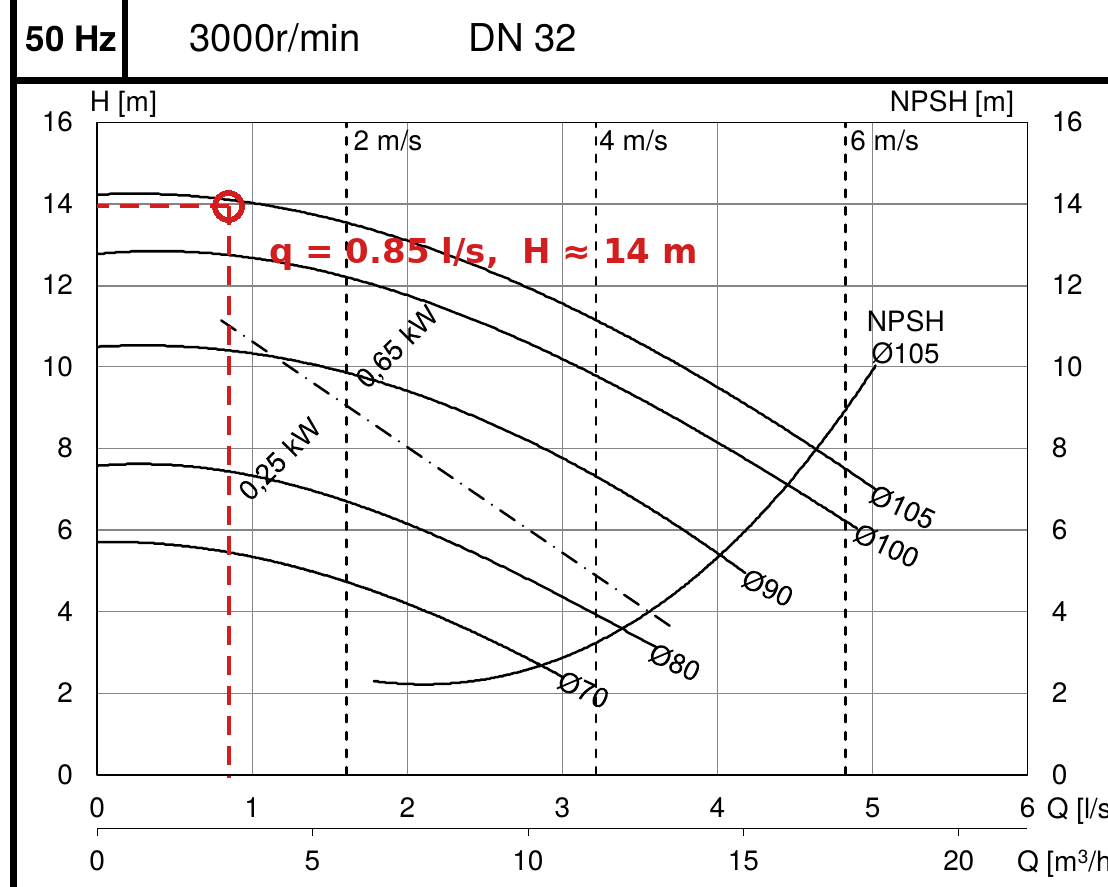
\includegraphics[width=0.8\textwidth]{Pictures/Pump_Curve_Operating_Point.png}
    \caption{Pump curve of the Kolmeks L-32A/2 (50\,Hz) with the operating point $q = 0.85\,\text{l/s}$, $H \approx 14\,\text{m}$ marked in red. \textit{Note.} Adapted from Kolmeks (2012).}
    \label{fig:pump}
\end{figure}

Converting head to pressure ($\rho = 1000\,\text{kg/m}^3$, $g = 9.81\,\text{m/s}^2$):
\begin{equation}
    p_{pump} = \rho g H = 1000 \cdot 9.81 \cdot 14 = 137\,340\,\text{Pa} \approx 1.37\,\text{bar}
\end{equation}
\begin{equation}
    \Delta p_0 = \rho g H_0 = 1000 \cdot 9.81 \cdot 14.2 = 139\,302\,\text{Pa} \approx 1.39\,\text{bar}
\end{equation}

\subsection{Pressure Loss Between Pump and Valve}
All components between the pump discharge and the valve inlet that cause pressure loss were identified from the P\&I diagram and the piping isometry (Table~\ref{tab:loss}): $2.38\,\text{m}$ of straight pipe (segments of $20$, $75$, $25$, $37$, $31$ and $50\,\text{cm}$), six $90^\circ$ elbows ($r = 8\,\text{cm}$), the flowmeter CF202, the pressure transmitter CP202 and the temperature sensor CT202. The three manual block valves LAA01AA006, LAA01AA101 and LAA01AA007 are located on the suction side of the pump and therefore do not belong to this section.

Flow velocity and Reynolds number in the DN\,32 pipe:
\begin{equation}
    v = \frac{4q}{\pi d^2} = \frac{4 \cdot 0.85\cdot 10^{-3}}{\pi \cdot 0.032^2} \approx 1.06\,\text{m/s}, \qquad
    Re = \frac{v d}{\nu} = \frac{1.06 \cdot 0.032}{0.893\cdot 10^{-6}} \approx 3.8\cdot 10^{4}
\end{equation}
The dynamic pressure is $\rho v^2/2 = 559\,\text{Pa}$. The friction factor follows from the Haaland equation (Haaland, 1983) with $\varepsilon/d = 0.046/32 = 1.44\cdot 10^{-3}$:
\begin{equation}
    \frac{1}{\sqrt{f}} = -1.8 \log_{10}\!\left[\left(\frac{\varepsilon/d}{3.7}\right)^{1.11} + \frac{6.9}{Re}\right] \;\Rightarrow\; f \approx 0.026
\end{equation}
The pressure loss of the straight pipe and of the fittings is
\begin{align}
    \Delta p_{pipe} &= f\,\frac{L}{d}\,\frac{\rho v^2}{2} = 0.026 \cdot \frac{2.38}{0.032} \cdot 559 \approx 1.08\,\text{kPa} \\
    \Delta p_{elbows} &= n\,K\,\frac{\rho v^2}{2} = 6 \cdot 0.25 \cdot 559 \approx 0.84\,\text{kPa}
\end{align}
The temperature sensor is the only intrusive element. It is treated as a cylinder in cross flow (drag coefficient $C_D \approx 1.2$) with the well diameter $d_w = 11\,\text{mm}$ taken from the SKS well catalogue (SKS Automaatio, 2015) and a conservative immersion length $L_w = d = 32\,\text{mm}$ (well reaching the opposite wall):
\begin{equation}
    \Delta p_{CT202} = C_D\,\frac{\rho v^2}{2}\,\frac{d_w L_w}{A} = 1.2 \cdot 559 \cdot \frac{0.011 \cdot 0.032}{8.04\cdot 10^{-4}} \approx 0.29\,\text{kPa}
\end{equation}

\begin{table}[H]
\centering
\caption{Pressure loss between pump discharge and valve inlet at $q = 0.85\,\text{l/s}$}
\label{tab:loss}
\small
\begin{tabularx}{\textwidth}{@{}cp{3.6cm}Xrp{2.6cm}@{}}
\toprule
No. & Component & Basis & $\Delta p$ [bar] & Source \\
\midrule
1 & Straight pipe, 2.38\,m, DN\,32 & $f = 0.026$, $L/d = 74.4$ & 0.011 & Haaland (1983) \\
2 & $6\times$ elbow $90^\circ$, $r/d = 2.5$ & $K = 0.25$ each, $\sum K = 1.5$ & 0.008 & Crane Co. (2009) \\
3 & Flowmeter CF202 (ProcessMaster 300) & Electromagnetic, no internals in flow path; $K \approx 0$ (assumed) & $\approx 0$ & ABB (n.d.) \\
4 & Pressure transmitter CP202 (SATRON VT) & Pressure tapping, no through-flow, $K \approx 0$ & $\approx 0$ & Satron Instruments (2015) \\
5 & Temperature sensor CT202 (SKS Pt100) & Well $\varnothing 11\,\text{mm}$, $L_w = 32\,\text{mm}$, $C_D = 1.2$ & 0.003 & SKS Automaatio (2015) \\
\midrule
 & \multicolumn{2}{l}{\textbf{Total pump $\rightarrow$ valve}} & \textbf{0.022} & \\
\bottomrule
\end{tabularx}
\end{table}

As a cross-check, the web calculator \textit{Pressure Drop Online} (Pressure Drop Online, n.d.) gives $0.021\,\text{bar}$ for the pipe and the six elbows at $q = 0.85\,\text{l/s}$ (DN\,32), compared with $0.019\,\text{bar}$ from rows 1 and 2 of Table~\ref{tab:loss}. The total loss of about $0.02\,\text{bar}$ is small compared with the pump pressure of $1.37\,\text{bar}$; practically the entire pump pressure remains for the control valve.

Downstream of the valve, the short $0.12\,\text{m}$ pipe with one elbow discharges into the tank:
\begin{equation}
    \Delta p_{down} = 0.026\cdot\frac{0.12}{0.032}\cdot 559 + 0.25\cdot 559 \approx 0.002\,\text{bar}
\end{equation}

\subsection{Pressure Drop Across the Valve and \texorpdfstring{$DP_m$}{DPm}}
Since the static head difference is zero, the pump pressure is dissipated in the pipework and in the valve:
\begin{equation}
    \Delta p_{valve} = p_{pump} - \Delta p_{pump\rightarrow valve} - \Delta p_{down} = 1.373 - 0.022 - 0.002 \approx 1.35\,\text{bar}
\end{equation}
With the assumed tank pressure of $0.2\,\text{barG}$ this gives a valve inlet pressure of $0.2 + 1.373 - 0.022 \approx 1.55\,\text{barG}$ and a valve outlet pressure of $0.2\,\text{barG}$. The inlet pressure is below the design pressure of the existing valve ($500\,\text{kPa}$).

According to the Flow Control Manual (Valmet, 2022, eq.\,10) the process pressure ratio $DP_m$ is the valve pressure drop at maximum flow divided by the pressure drop across the closed valve:
\begin{equation}
    DP_m = \frac{\Delta p_m}{\Delta p_0} = \frac{1.35}{1.39} \approx 0.97
\end{equation}
This is far above the rule-of-thumb value $DP_m = 0.30$ for liquid piping (Valmet, 2022, eq.\,15), which is also the default of the sizing software. The reason is the very short piping with low losses together with a flat pump curve: the valve takes almost the entire pump pressure. Consequently the installed flow characteristic follows the inherent characteristic much more closely than for a typical piping system. $DP_m = 0.97$ therefore has to be entered into the Nelprof process model (Section~\ref{sec:nelprof}).

\subsection{Required Flow Coefficient}
\begin{equation}
    C_v = \frac{q}{N_1\sqrt{\Delta p_{valve}/G_f}} = \frac{3.06\,\text{m}^3/\text{h}}{0.865\cdot\sqrt{1.35/1.0}} \approx 3.04
\end{equation}
with $N_1 = 0.865$ for $q$ in $\text{m}^3/\text{h}$ and $\Delta p$ in bar, and specific gravity $G_f = 1.0$.

% ---------------------------------------------------------
\section{Sizing Results (Nelprof)}
\label{sec:nelprof}
The process data of Table~\ref{tab:nelprof_in} were entered into Valmet Nelprof for two DN\,25 valve alternatives (Appendix~A, Figures~\ref{fig:setup_re} and~\ref{fig:setup_m1}). The current Jamesbury valve was evaluated with its direct equivalent, the Valmet M1-series. The process pressure ratio was set to the calculated $DP_m = 0.97$ in the process model settings of the charts section \nel{add screenshot of this setting}.

\begin{table}[H]
\centering
\caption{Nelprof input data}
\label{tab:nelprof_in}
\small
\begin{tabular}{@{}ll@{}}
\toprule
Parameter & Value \\
\midrule
Liquid flow rate & $0.85\,\text{l/s}$ \\
Inlet temperature & $25^\circ\text{C}$ \\
Inlet pressure / outlet pressure & $1.55\,\text{barG}$ / $0.20\,\text{barG}$ \\
Pressure difference $\Delta p_{valve}$ & $1.35\,\text{bar}$ \\
Vapour pressure & $0.0317\,\text{bar(a)}$ \\
Pipe size (inlet / outlet) & $32\,\text{mm}$ \\
Process pressure ratio $DP_m$ & $0.97$ \\
\bottomrule
\end{tabular}
\end{table}

\subsection{Alternative 1: RE-Series Segmented Ball Valve}
According to the manufacturer's documentation, the RE-series is a V-port segment valve with an equal-percentage inherent characteristic and an optional reduced $C_v$ trim for DN\,25 valves to control very low flows (Valmet, 2025). The reduced trim (reduction 2, maximum capacity $5\,C_v$) was selected to match the low required capacity.
\begin{itemize}
    \item \textbf{Required capacity ($C_v$):} \REcv\ (hand calculation: 3.04)
    \item \textbf{Travel / opening:} \REtravel\ (\REangle)
    \item \textbf{Predicted noise level:} \REnoise
    \item \textbf{Choked $\Delta p$:} \REchoked\ (no cavitation if $\Delta p = 1.35\,\text{bar}$ is below this value)
\end{itemize}

\subsection{Alternative 2: M1-Series Standard Ball Valve}
The standard M1-series ball valve (maximum capacity $105\,C_v$) was evaluated under the same process conditions.
\begin{itemize}
    \item \textbf{Required capacity ($C_v$):} \Mcv\ (hand calculation: 3.04)
    \item \textbf{Travel / opening:} \Mtravel\ (\Mangle)
    \item \textbf{Predicted noise level:} \Mnoise\ at the operating point (peak: \Mnoisepeak\ at \Mnoisepeaktravel\ travel)
    \item \textbf{Choked $\Delta p$:} \Mchoked
\end{itemize}

% ---------------------------------------------------------
\section{Graphical Analysis (Nelprof Charts)}
The charts in Figures~\ref{fig:inherent} to~\ref{fig:noise} show the hydrodynamic and control behaviour of the valves. The RE-series is displayed on top, the M1-series below it.

\subsection{Inherent Flow Characteristics}
\begin{figure}[H]
    \centering
    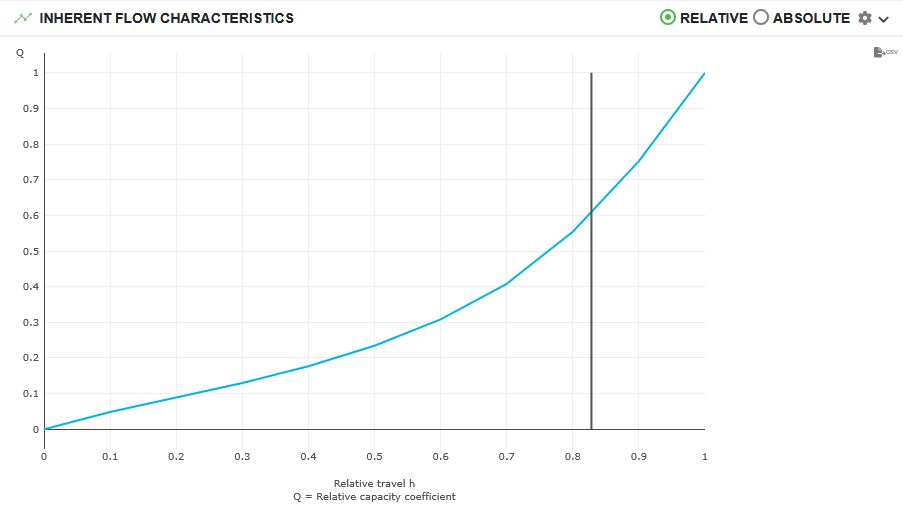
\includegraphics[width=0.9\textwidth]{Pictures Nelprof/RE_InherentFlowCharacteristics_Relative.png}
    \\[0.5cm]
    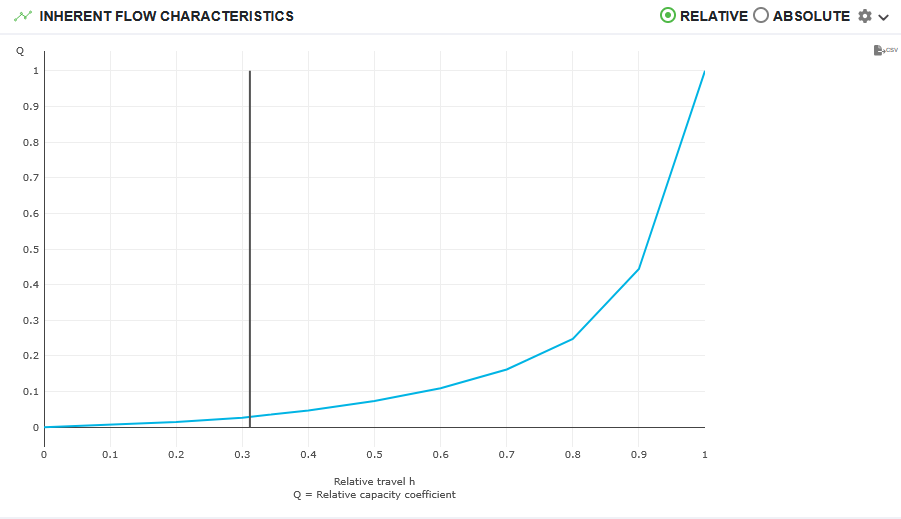
\includegraphics[width=0.9\textwidth]{Pictures Nelprof/M1_InherentFlowCharacteristics_Relative.png}
    \caption{Inherent flow characteristics (top: RE-series, bottom: M1-series). \textit{Note.} Nelprof output.}
    \label{fig:inherent}
\end{figure}
Figure~\ref{fig:inherent} shows the flow capacity of the valve as a function of relative travel at constant pressure drop. The RE-series (top) has the equal-percentage characteristic stated by the manufacturer (Valmet, 2025): at 50\,\% travel the relative capacity is 23.3\,\%, at 80\,\% travel 55.4\,\%. The M1-series (bottom) has a total capacity of $105.0\,C_v$ and is very strongly oversized for a required capacity of about $3\,C_v$. Its curve is flat over the first two thirds of the travel and rises steeply only close to the fully open position. The required capacity is therefore reached at a small relative opening around one third of the travel, where small travel changes cause large relative capacity changes.

\subsection{Installed Flow Characteristics}
\begin{figure}[H]
    \centering
    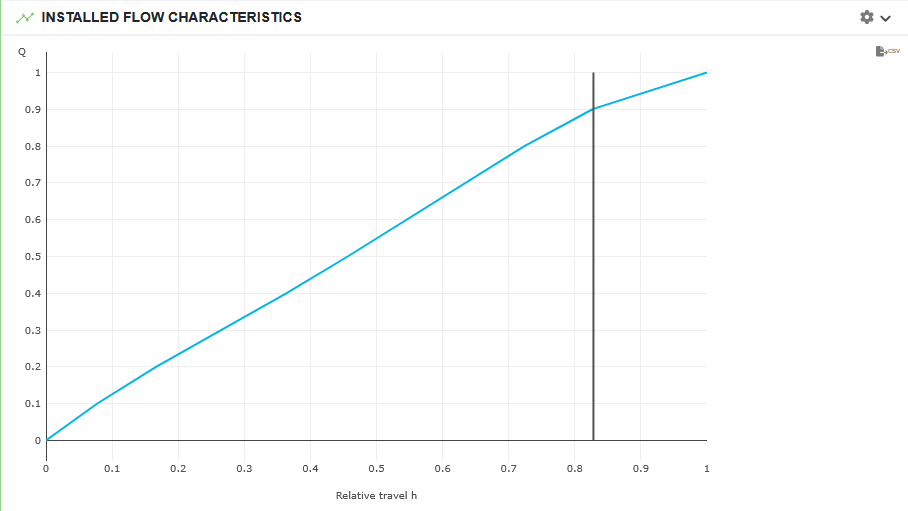
\includegraphics[width=0.9\textwidth]{Pictures Nelprof/RE_InstalledFlowCharacteristics.png}
    \\[0.5cm]
    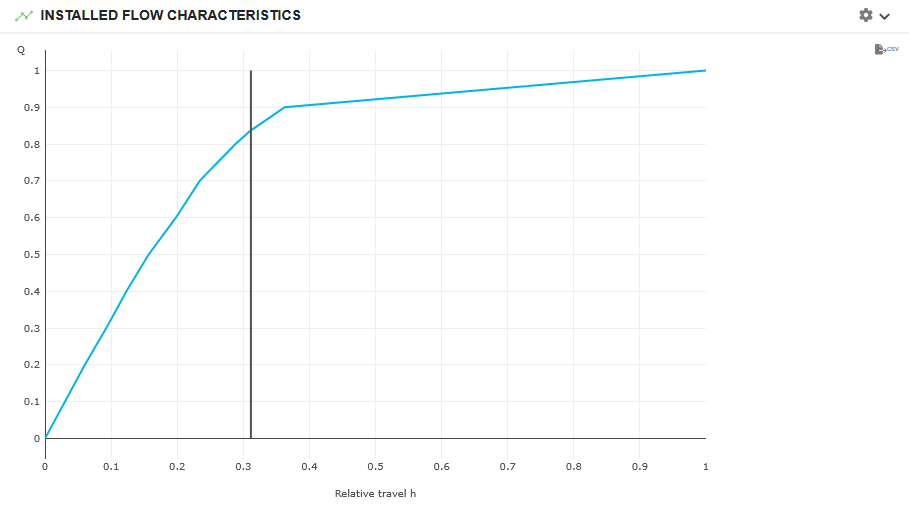
\includegraphics[width=0.9\textwidth]{Pictures Nelprof/M1_InstalledFlowCharacteristics.png}
    \caption{Installed flow characteristics (top: RE-series, bottom: M1-series, $DP_m = 0.97$). \textit{Note.} Nelprof output.}
    \label{fig:installed}
\end{figure}
The installed characteristic in Figure~\ref{fig:installed} includes the pressure behaviour of the process. Because $DP_m$ is close to 1, the installed characteristic of the RE-series stays close to its equal-percentage inherent characteristic (JAMK University of Applied Sciences, 2024; Valmet, 2022): travel 0.5 yields a relative flow of \REflowhalf\ and travel 0.8 a relative flow of \REflowhigh. The oversized M1-series (bottom) reaches 80\,\% of the installed flow at \Mtraveleighty\ travel and 90\,\% at \Mtravelninety\ travel, so the usable control range is compressed into the first third of the travel and the remaining travel is of no use for this process.

\subsection{Installed Gain}
\begin{figure}[H]
    \centering
    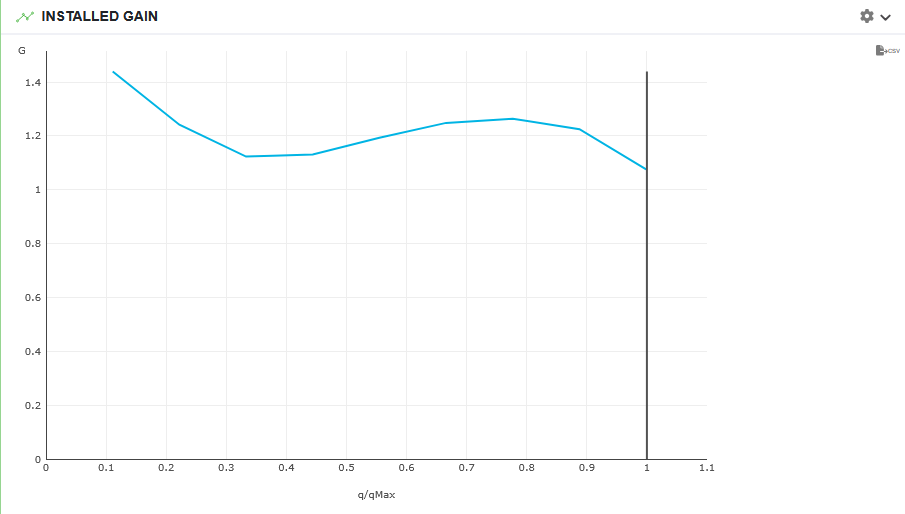
\includegraphics[width=0.9\textwidth]{Pictures Nelprof/RE_InstalledGain.png}
    \\[0.5cm]
    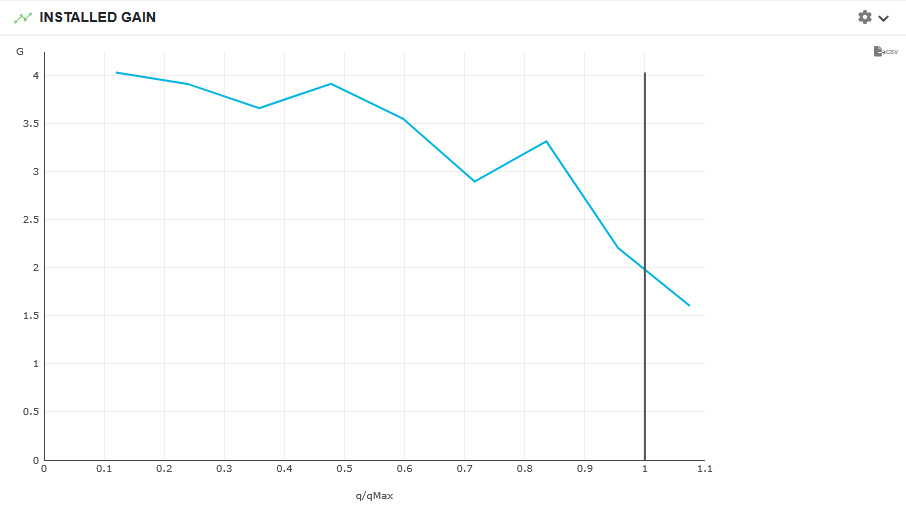
\includegraphics[width=0.9\textwidth]{Pictures Nelprof/M1_InstalledGain.png}
    \caption{Installed gain (top: RE-series, bottom: M1-series). \textit{Note.} Nelprof output.}
    \label{fig:gain}
\end{figure}
The installed gain $G = dQ_p/dh$ describes the sensitivity of the flow to a change in valve position. According to the Flow Control Manual (Valmet, 2022, eq.\,13 and 14) the loop behaves similarly at all operating points if $G_{max}/G_{min} < 2$ and the relative gain does not fall below $0.5$.

For the RE-series (Figure~\ref{fig:gain}, top) the gain varies between \REgmin\ and \REgmax, i.e.\ $G_{max}/G_{min} = $ \REratio\ \nel{state whether criterion $<2$ is met}. For the M1-series (bottom) the gain varies between \Mgmin\ and \Mgmax\ with \Mgop\ at the operating point, $G_{max}/G_{min} = $ \Mratio\ \nel{state whether criterion $<2$ is met}. Since the M1 gain is in addition at a high absolute level, a small change of valve position causes a large change of flow, which promotes control loop oscillation and makes tuning of the PID controller difficult (Valmet, 2022). \nel{Discuss: with DP$_m \approx 1$ the equal-percentage characteristic of the RE gives a gain that rises with flow; evaluate against the result above.}

\subsection{Installed Pressure Level}
\begin{figure}[H]
    \centering
    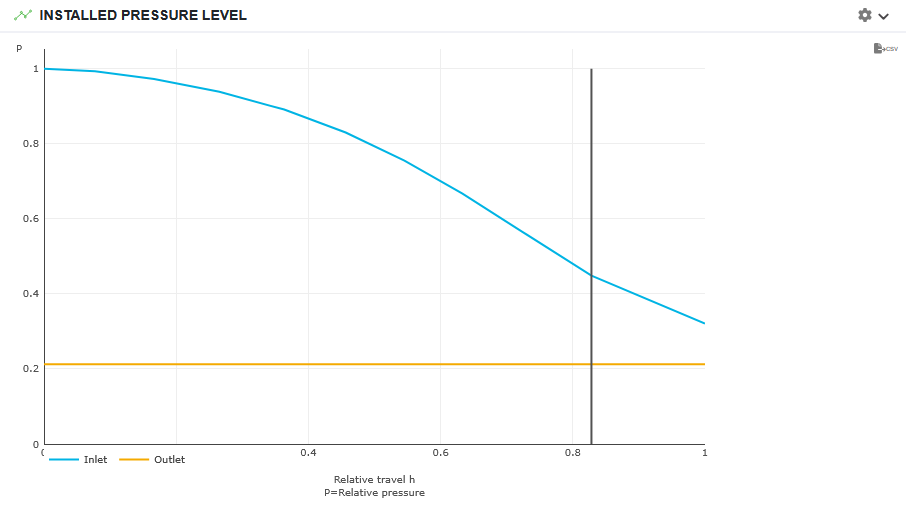
\includegraphics[width=0.9\textwidth]{Pictures Nelprof/RE_InstalledPressureLevel.png}
    \\[0.5cm]
    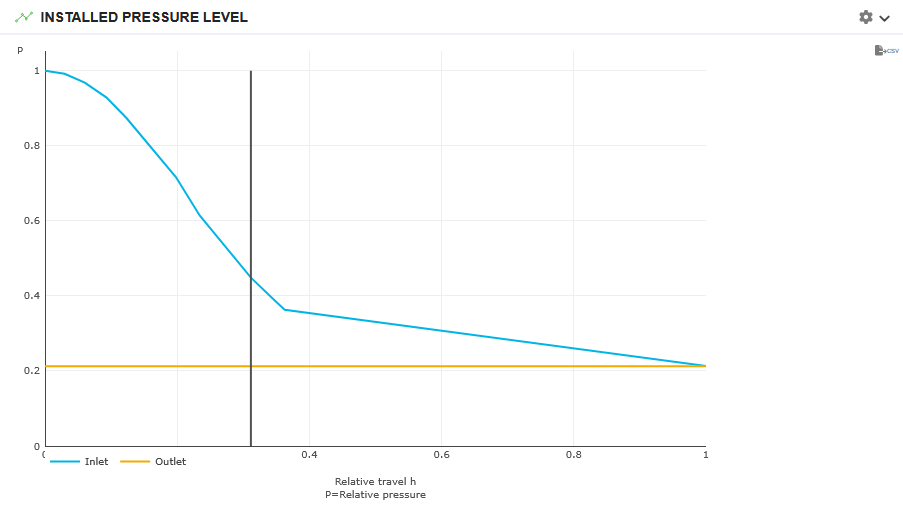
\includegraphics[width=0.9\textwidth]{Pictures Nelprof/M1_InstalledPressureLevel.png}
    \caption{Installed pressure level (top: RE-series, bottom: M1-series). \textit{Note.} Nelprof output.}
    \label{fig:pressure}
\end{figure}
Figure~\ref{fig:pressure} shows the relative upstream and downstream pressure of the valve as a function of travel. With increasing opening the valve inlet pressure falls from 1.0 (closed valve) to \REpinfull\ (RE) and \Mpinfull\ (M1) at the fully open position, while the outlet pressure remains constant. In both cases the pressure downstream of the valve stays far above the vapour pressure of $0.0317\,\text{bar(a)}$, so flashing does not occur (Valmet, 2022).

\subsection{Installed Noise}
\begin{figure}[H]
    \centering
    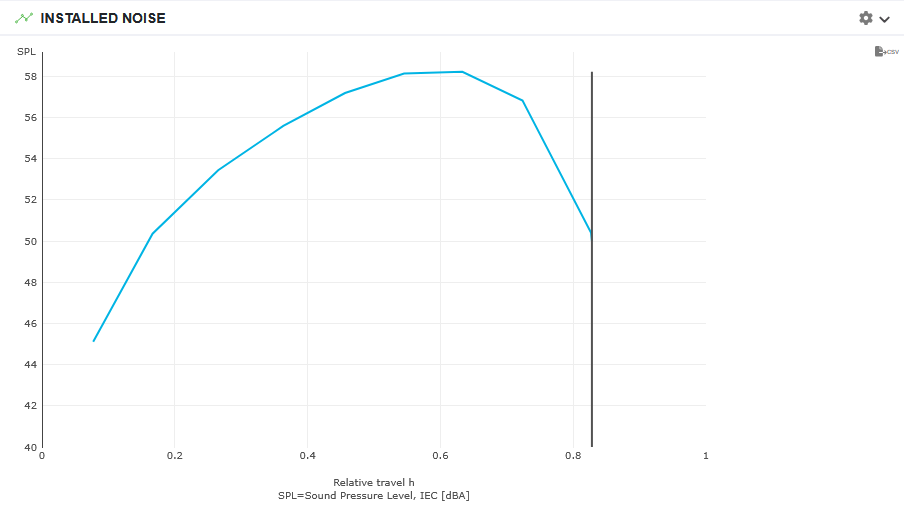
\includegraphics[width=0.9\textwidth]{Pictures Nelprof/RE_InstalledNoise.png}
    \\[0.5cm]
    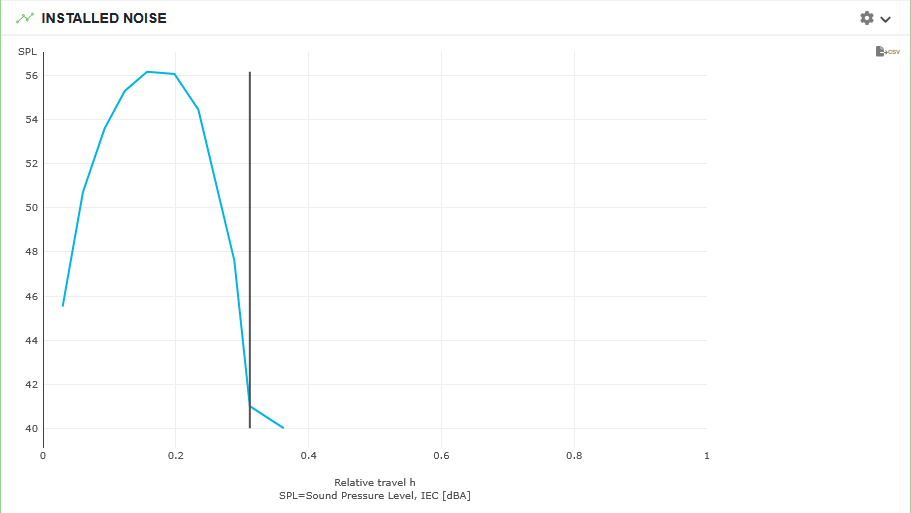
\includegraphics[width=0.9\textwidth]{Pictures Nelprof/M1_InstalledNoise.png}
    \caption{Installed hydrodynamic noise (top: RE-series, bottom: M1-series). \textit{Note.} Nelprof output.}
    \label{fig:noise}
\end{figure}
Hydrodynamic noise is an indicator of cavitation intensity. In Figure~\ref{fig:noise} the RE-series peaks at \REnoisepeak\ at \REnoisepeaktravel\ travel and reaches \REnoise\ at the operating point; the M1-series peaks at \Mnoisepeak\ at \Mnoisepeaktravel\ travel and reaches \Mnoise\ at the operating point. The noise limit given in the Flow Control Manual for this application is $80\,\text{dBA}$ (Valmet, 2022). \nel{check wording/limit against the manual table}. Both valves stay clearly below this limit; in addition $\Delta p_{valve} = 1.35\,\text{bar}$ is below the choked pressure drop of both valves, so no cavitation is expected.

% ---------------------------------------------------------
\section{Comparative Evaluation and Conclusions}

\subsection{Valve Performance Comparison}
The currently installed valve type (M1-series ball valve) offers tight shut-off and a very high maximum capacity, which is the opposite of what a throttling duty at about $3\,C_v$ requires (JAMK University of Applied Sciences, 2024). With $105\,C_v$ the valve works at about \Mtravel\ travel, reaches 90\,\% of the installed flow at \Mtravelninety\ travel and shows a high installed gain (up to \Mgmax; $G_{max}/G_{min}$ = \Mratio). This leaves little resolution for the controller.

The RE-series segmented ball valve with reduced trim ($5\,C_v$ maximum) matches the required capacity much better. It works at \REtravel\ travel with an installed gain between \REgmin\ and \REgmax\ ($G_{max}/G_{min}$ = \REratio). \nel{Critical remark: discuss the remaining flow reserve at the operating travel (valve travel at design flow) and the consequence of DP$_m \approx 0.97$ for the equal-percentage characteristic.}

\subsection{Product Documentation of the Selected Valve}
The manufacturer's documentation (Valmet, 2025) describes the RE-series as an integrally flanged V-port segment valve in quarter-turn design with equal-percentage inherent characteristic. The reduced $C_v$ trim is available for DN\,25 valves only and is intended for very low flows, which matches the required capacity of about $3\,C_v$. Standard units are supplied with diaphragm or cylinder actuators and ND9000 intelligent valve controllers.

\subsection{Actuator}
The installed AUMA SGR\,04.3 is an electric part-turn actuator. The manufacturer's standard configuration for the RE-series uses a pneumatic actuator with an ND9000 valve controller (Valmet, 2025). Changing the actuator is a secondary recommendation; the valve selection does not depend on it.

\subsection{Final Verdict}
Based on the process data, the pressure loss calculation between pump and valve ($\Delta p_{valve} = 1.35\,\text{bar}$, $DP_m = 0.97$) and the Nelprof analysis, the \textbf{RE-series segmented ball valve (DN\,25, reduced trim)} is more suitable than the M1-series ball valve for this application, because the M1 is heavily oversized and works in a small part of its travel with a high installed gain. \nel{Confirm after the Nelprof re-run.}

% ---------------------------------------------------------
\section*{Declaration on the Use of Artificial Intelligence}
In accordance with the JAMK reporting guidelines it is declared that generative AI was used as a support tool. AI was used for language checking, for formatting the LaTeX document and for reviewing the calculation approach (pressure balance, $DP_m$ definition) and the consistency of the report. The pipe friction calculation, the component losses, the pressure drop across the valve, $DP_m$ and $C_v$ (Section~3) were calculated and checked by the author; the pipe loss was cross-checked with \textit{Pressure Drop Online}. All sizing was performed by the author in Nelprof, and the interpretation of the results and the valve selection are the author's own. The author is fully responsible for the technical content.

% ---------------------------------------------------------
\clearpage
\section*{References}
\addcontentsline{toc}{section}{References}
\begingroup
\setlength{\parindent}{-1.25cm}
\setlength{\leftskip}{1.25cm}
\setlength{\parskip}{0.5em}
\raggedright
ABB. (n.d.). \textit{ProcessMaster FEP300 electromagnetic flowmeter} (Data sheet DS/FEP300-EN, Rev. K). \url{https://library.e.abb.com/public/5996486236d6463ab3375fb48033fd17/DS_FEP300_EN_K.pdf}

Crane Co. (2009). \textit{Flow of fluids through valves, fittings, and pipe} (Technical Paper No. 410).

Haaland, S. E. (1983). Simple and explicit formulas for the friction factor in turbulent pipe flow. \textit{Journal of Fluids Engineering, 105}(1), 89--90.

JAMK University of Applied Sciences. (n.d.). \textit{Process diagram 35899, rev. 7} [P\&I diagram]. Field Devices and Instrumentation.

JAMK University of Applied Sciences. (2024). \textit{Valve structures and control valves} [Learning material]. Field Devices and Instrumentation.

Kolmeks. (2012). \textit{Pump performance curve: L-32A/2 (105 mm impeller)}.

Pressure Drop Online. (n.d.). \textit{Pressure drop calculator} [Web application]. \nel{add URL and retrieval date}

Satron Instruments. (2015). \textit{SATRON VT painel\"ahetin} [Data sheet].

SKS Automaatio. (2015). \textit{L\"amp\"otila-anturi: Valmistusohjelma ja anturityypit} [Data sheet].

Valmet. (n.d.). \textit{Nelprof} [Computer software]. \nel{add URL and retrieval date}

Valmet. (2022). \textit{Flow control manual} (6th ed.). Neles Finland Oy.

Valmet. (2025). \textit{Neles V-port segment valve RE-series} (Brochure 13R24EN). \url{https://www.valmet.com/globalassets/sharepoint/imported/3r24en.pdf}
\endgroup

% ---------------------------------------------------------
\clearpage
\appendix
\section{Nelprof Setup Screenshots}
\begin{figure}[H]
    \centering
    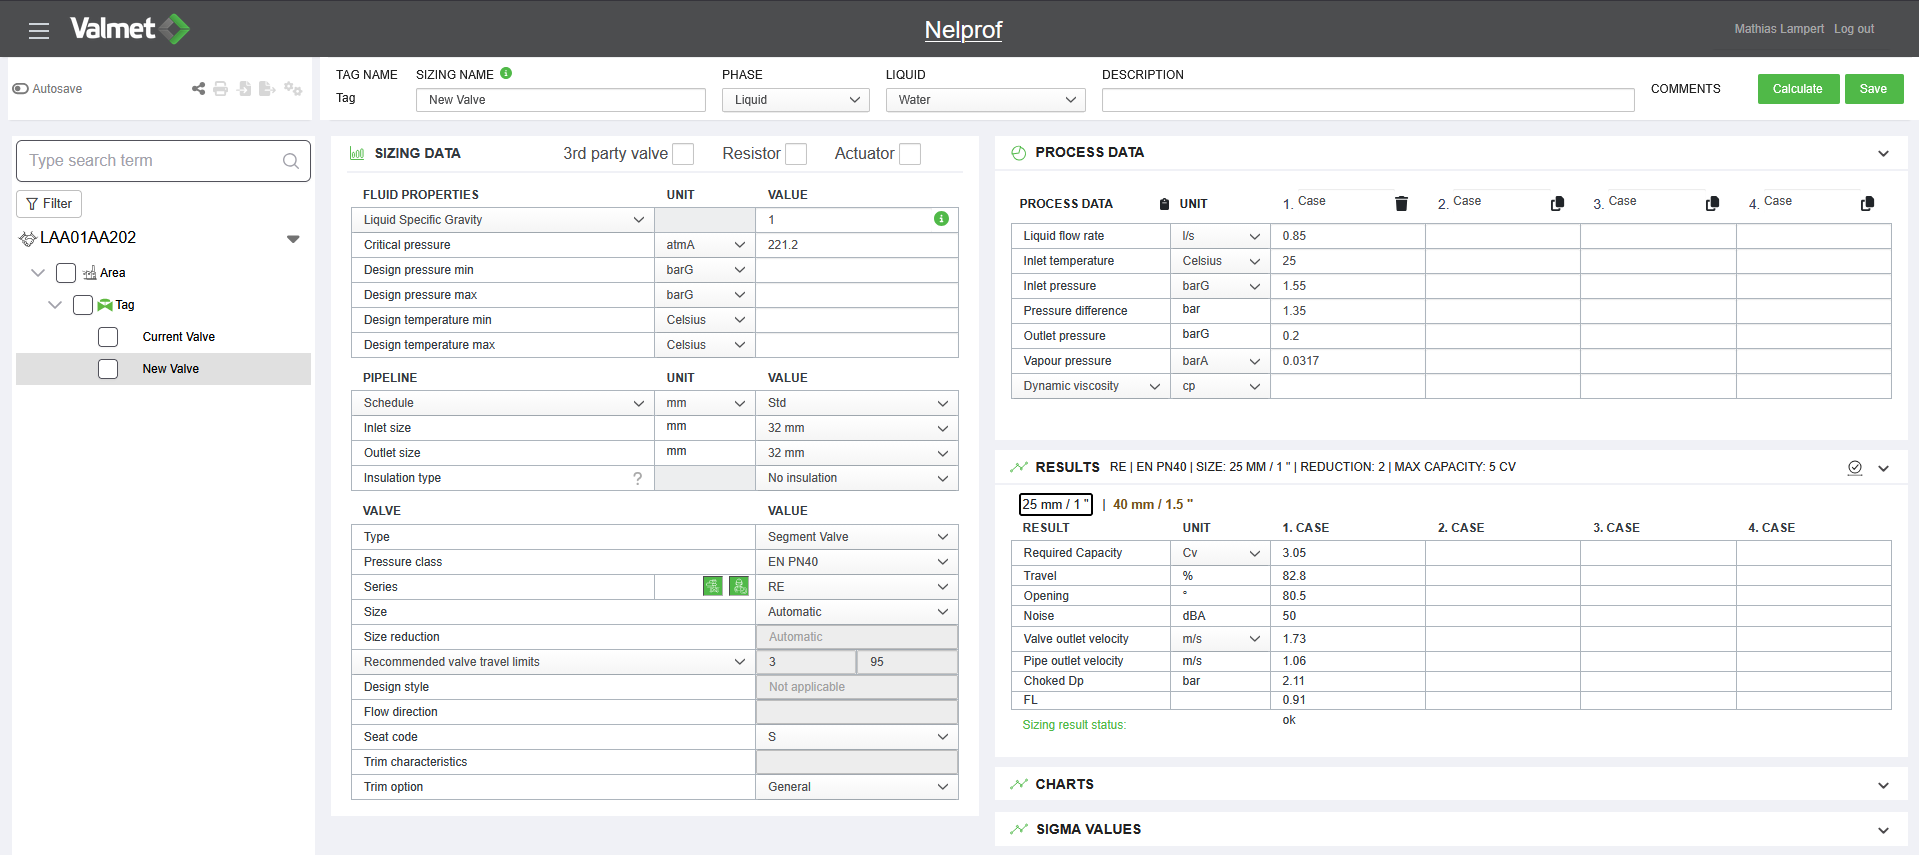
\includegraphics[width=\textwidth]{Pictures Nelprof/RE_Nelprof_Setup.png}
    \caption{Nelprof setup and results, RE-series. \textit{Note.} Nelprof output.}
    \label{fig:setup_re}
\end{figure}
\begin{figure}[H]
    \centering
    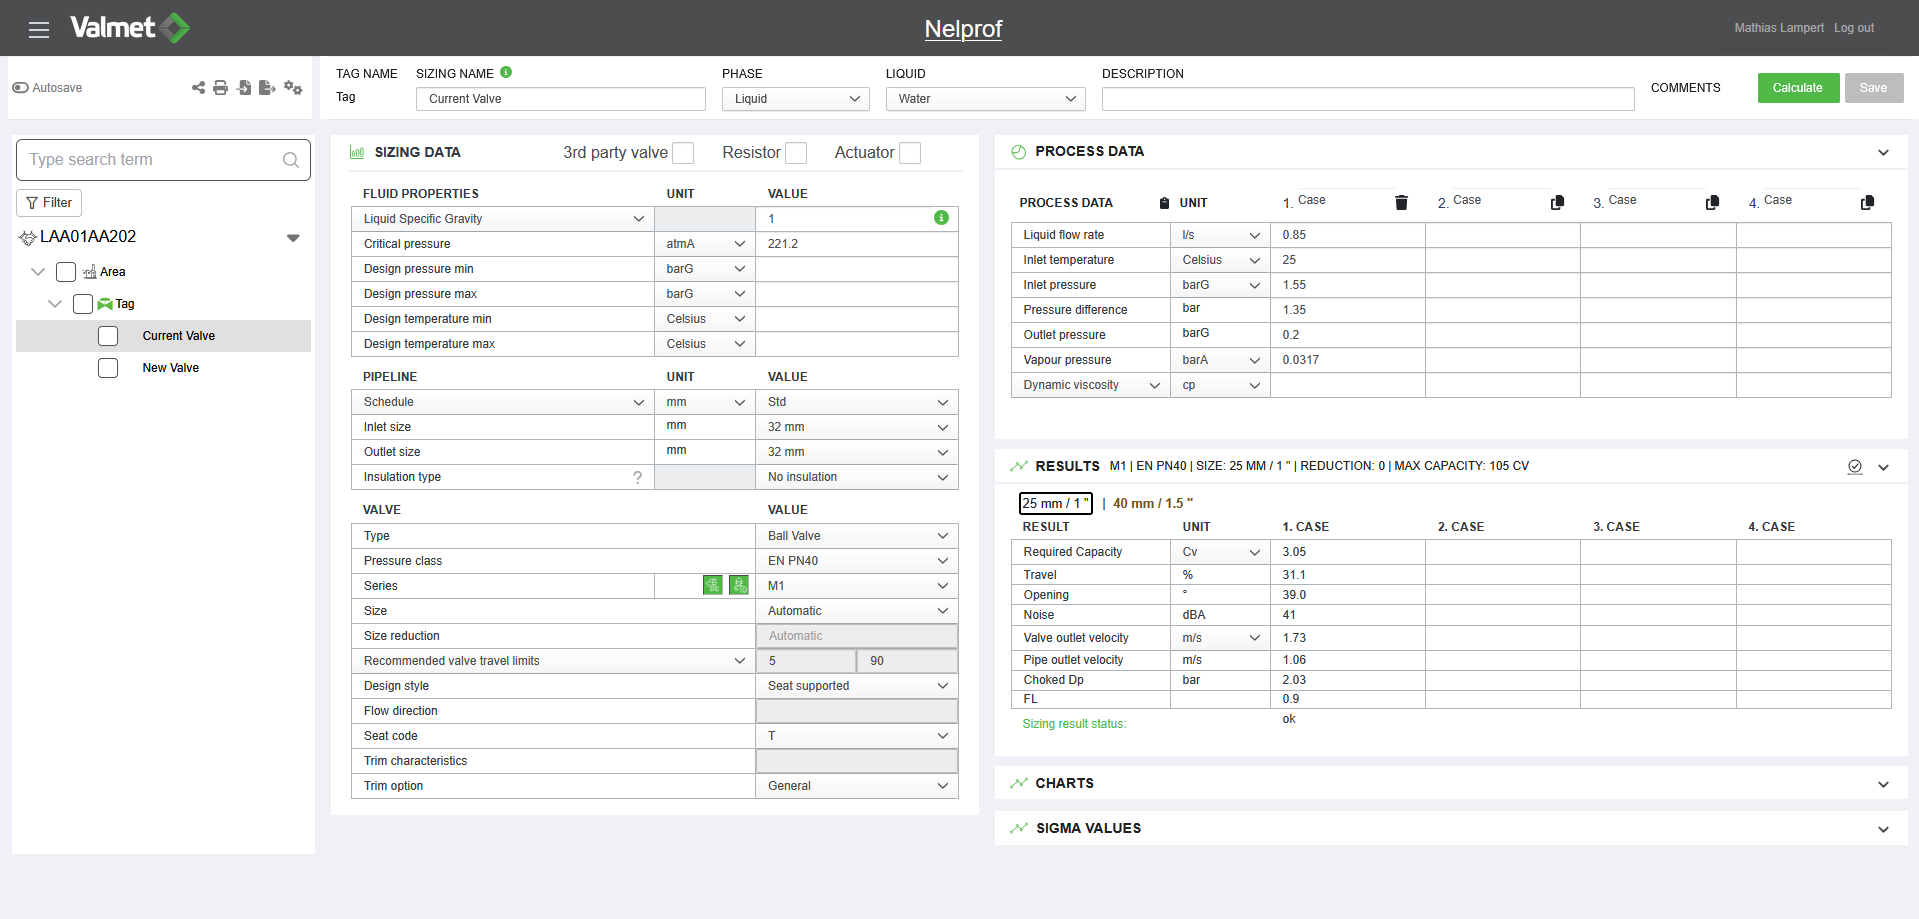
\includegraphics[width=\textwidth]{Pictures Nelprof/M1_Nelprof_Setup.png}
    \caption{Nelprof setup and results, M1-series. \textit{Note.} Nelprof output.}
    \label{fig:setup_m1}
\end{figure}

\end{document}